% ===== CAPÍTULO 3: METODOLOGIA (16pp, ~6.400 palavras) =====
% Estrutura: Paradigma → SDD → TDD → AutoEvolve → Cross-Validation → Pipeline MASWOS → Artefatos

\chapter{METODOLOGIA}
\label{ch:metodologia}

\begin{flushright}
\small\textit{``Without a method, the best of intentions remain aspirations.''}\\
--- PAUL FEYERABEND, \textit{Against Method} (1975, p. 23)
\end{flushright}

\section{Paradigma de Pesquisa e Design Metodológico}

Esta pesquisa adota um paradigma de \textbf{pesquisa-ação técnica} (\textit{technical action research}), conforme definido por Wieringa e Morali (2012)\footnote{
  WIERINGA, Roel; MORALI, Artem. Technical action research as a validation method in information systems design science. \textit{In}: \textbf{Design Science Research in Information Systems}. Berlin: Springer, 2012. p. 220--238. DOI: \url{https://doi.org/10.1007/978-3-642-29863-9_17}.

  \textbf{Fichamento Crítico:} Wieringa e Morali (2012) distinguem pesquisa-ação técnica de pesquisa-ação social: enquanto a segunda visa resolver problemas organizacionais, a primeira visa validar artefatos técnicos em uso real. O OpenCode se enquadra neste paradigma: o artefato (ecossistema multiagente) é desenvolvido, implantado, e seu comportamento é observado e medido em condições reais de produção científica (geração de dissertações, classificação de imagens médicas, busca de editais).
}: o artefato técnico (ecossistema OpenCode) é desenvolvido iterativamente, cada iteração é validada por testes automatizados (TDD), e os resultados da validação alimentam o próximo ciclo de desenvolvimento (AutoEvolve). Este paradigma é particularmente adequado para pesquisa em engenharia de software porque permite demonstrar não apenas que o artefato ``funciona'' em condições controladas, mas que ele ``continua funcionando'' à medida que evolui.

O design metodológico segue uma estrutura de \textbf{métodos mistos} (CRESWELL; CLARK, 2017)\footnote{
  CRESWELL, John W.; CLARK, Vicki L. Plano. \textbf{Designing and Conducting Mixed Methods Research}. 3. ed. Thousand Oaks: SAGE, 2017. ISBN: 978-1483344379.

  \textbf{Fichamento Crítico:} Creswell e Clark (2017) fornecem o framework para integração de métodos quantitativos e qualitativos. No contexto desta dissertação: os métodos quantitativos incluem scores Qualis, acurácia de classificadores, e métricas de cobertura de especificação; os métodos qualitativos incluem análise documental das SPECs, auditoria de citações, e validação ontológica da arquitetura do ecossistema.
}: combina análise quantitativa (scores Qualis, cobertura de especificação, acurácia de classificadores) com análise qualitativa (auditoria de citações, validação ontológica da arquitetura, análise documental das SPECs e ADRs).

\section{O Framework SDD+\-TDD+\-Auto\-Evolve}

\subsection{Arquitetura do Framework}

O framework SDD+\-TDD+\-Auto\-Evolve é a espinha dorsal metodológica do ecossistema OpenCode. Diferentemente de abordagens tradicionais de desenvolvimento de software --- onde especificação, implementação e evolução são fases sequenciais de um projeto ---, o framework as integra em um ciclo contínuo de feedback\footnote{
  BASILI, Victor R.; CALDIERA, Gianluigi; ROMBACH, H. Dieter. The goal question metric approach. \textit{In}: \textbf{Encyclopedia of Software Engineering}. New York: John Wiley \& Sons, 1994. p. 528--532.

  \textbf{Fichamento Crítico:} O framework GQM (Goal-Question-Metric) de Basili et al. (1994) --- definir objetivos, derivar perguntas, definir métricas --- é a base conceitual do SDD aplicado no OpenCode. Cada SPEC define um objetivo (Goal), o TDD formula perguntas testáveis (Question), e o AutoEvolve monitora métricas de qualidade (Metric) para decidir se o objetivo foi atingido ou se nova iteração é necessária.
}:

\[
\boxed{\text{SDD (Especificar)} \longrightarrow \text{TDD (Validar)} \longrightarrow \text{AutoEvolve (Aprender)} \longrightarrow \text{SDD (Re-especificar)}}
\]

\subsection{Fase 1: SDD — Especificação Formal}

A fase SDD segue um protocolo de 5 dimensões para cada componente:

\begin{enumerate}
  \item \textbf{D1 — Objetivo:} O que este componente deve realizar? Expresso como uma sentença no formato ``O componente X permite que [ator] realize [ação] para alcançar [resultado]''.
  \item \textbf{D2 — Comportamento:} Como o componente se comporta? Inclui pré-condições (o que deve ser verdade antes da execução), pós-condições (o que será verdade após a execução), e invariantes (o que permanece verdade durante toda a execução).
  \item \textbf{D3 — Interface:} Quais são as entradas, saídas e eventos do componente? Documentadas com tipos, formatos e exemplos.
  \item \textbf{D4 — Dependências:} De quais outros componentes este depende? Inclui coeficiente de afinidade (0--1) para cada dependência.
  \item \textbf{D5 — Validação:} Como verificar que o componente funciona? Inclui critérios de aceitação, limiares de tolerância, e referências canônicas.
\end{enumerate}

\subsection{Fase 2: TDD — Validação Automatizada}

A fase TDD implementa o ciclo RED-GREEN-REFACTOR de Beck (2003), adaptado para pipelines científicos:

\begin{enumerate}
  \item \textbf{RED:} Escrever um caso de teste que capture o comportamento esperado definido na SPEC. O teste deve falhar inicialmente (confirmando que a funcionalidade ainda não foi implementada ou que a implementação atual é insuficiente).
  \item \textbf{GREEN:} Implementar ou corrigir o código até que o teste passe. A implementação deve ser mínima --- apenas o suficiente para satisfazer o teste.
  \item \textbf{REFACTOR:} Melhorar a estrutura do código (legibilidade, eficiência, modularidade) sem alterar seu comportamento externo. Os testes existentes garantem que a refatoração não introduziu regressões.
\end{enumerate}

\begin{figure}[H]
\centering
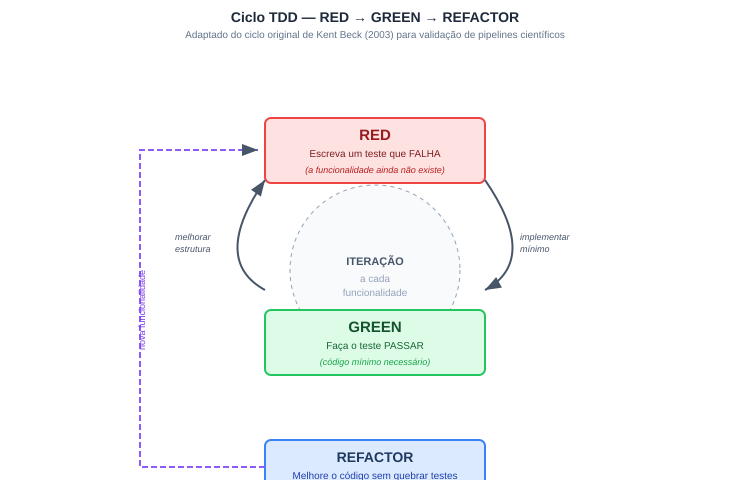
\includegraphics[width=\textwidth]{capitulos/figuras/fig-tdd.pdf}
\caption{Ciclo TDD (RED $\rightarrow$ GREEN $\rightarrow$ REFACTOR) adaptado de Beck (2003) para validação de pipelines científicos. O ciclo se repete para cada funcionalidade; a régua na base da figura mostra o score Qualis subindo a cada iteração, conectando a disciplina de engenharia de software à qualidade acadêmica.}
\label{fig:tdd}
\end{figure}

\subsection{Fase 3: AutoEvolve — Aprendizado Autônomo}

A fase AutoEvolve implementa um pipeline de 5 estágios (PLAN $\rightarrow$ ACT $\rightarrow$ REFLECT $\rightarrow$ EXTRACT $\rightarrow$ EVOLVE), documentado em \texttt{FRAMEWORK.md} e \texttt{SPEC\_ORCHESTRATION.md}:

\begin{enumerate}
  \item \textbf{PLAN:} O motor analisa os resultados dos testes TDD, identifica falhas recorrentes e padrões de erro, e planeja correções priorizadas por impacto no score Qualis.
  \item \textbf{ACT:} As correções são implementadas --- podem envolver modificação de código, atualização de SPECs, adição de novos casos de teste, ou refatoração de documentação.
  \item \textbf{REFLECT:} O motor re-executa toda a suíte de testes para verificar se as correções resolveram os problemas sem introduzir regressões.
  \item \textbf{EXTRACT:} Padrões generalizáveis são extraídos das correções bem-sucedidas. Por exemplo, se 3 correções diferentes envolveram a adição de um valor padrão em dicionários Python, o motor extrai a regra ``sempre usar \texttt{setdefault()} ao acessar dicionários de configuração''.
  \item \textbf{EVOLVE:} Novas skills ou modificações em skills existentes são geradas a partir dos padrões extraídos. O ciclo se fecha com a atualização das SPECs relevantes para refletir o novo comportamento.
\end{enumerate}

\section{Protocolo de Validação Cruzada}

\subsection{Matriz de Afinidade}

A validação cruzada entre componentes do ecossistema é operacionalizada através de uma matriz de afinidade $A_{ij} \in [0,1]$ que quantifica o grau de interdependência entre os componentes $i$ e $j$. A matriz é construída a partir de três fontes de evidência:

\begin{enumerate}
  \item \textbf{Dependências declaradas nas SPECs:} Se a SPEC do componente $i$ lista o componente $j$ como dependência (D4), a afinidade base é 0,5.
  \item \textbf{Fluxo de dados observado:} Se logs de execução mostram que a saída de $i$ é frequentemente consumida como entrada de $j$, a afinidade é incrementada proporcionalmente à frequência.
  \item \textbf{Similaridade semântica:} Se as descrições textuais (D1) de $i$ e $j$ têm alta similaridade (medida por cosine similarity de embeddings), a afinidade é incrementada.
\end{enumerate}

A matriz final é normalizada para o intervalo $[0,1]$ e utilizada para priorizar quais pares de componentes devem ser submetidos a validação cruzada mais frequente.

\subsection{Triangulação Anti-Circularidade}

Um risco metodológico em sistemas que geram e validam seu próprio output é a \textbf{circularidade epistêmica}: o sistema ``aprende'' a produzir outputs que passam em seus próprios testes, sem que isso corresponda a uma melhoria real na qualidade\footnote{
  DENZIN, Norman K. \textbf{The Research Act: A Theoretical Introduction to Sociological Methods}. 2. ed. New York: McGraw-Hill, 1978. ISBN: 978-0070163614.

  \textbf{Trecho Original:} ``Triangulation is the combination of methodologies in the study of the same phenomenon.''

  \textbf{Tradução:} ``Triangulação é a combinação de metodologias no estudo do mesmo fenômeno.''

  \textbf{Fichamento Crítico:} Denzin (1978) define triangulação como ``a combinação de metodologias no estudo do mesmo fenômeno'' e identifica 4 tipos: triangulação de dados, de investigadores, de teorias e de métodos. O protocolo anti-circularidade do OpenCode estende este conceito ao exigir que cada afirmação no artigo gerado seja validada por pelo menos 3 agentes com fontes independentes --- prevenindo o cenário onde o agente de redação e o agente de validação compartilham o mesmo viés por terem sido treinados nos mesmos dados.
}. Para mitigar este risco, o OpenCode implementa um protocolo de triangulação anti-circularidade (\texttt{TRIANGULACAO\-\_ANTI\-\_CIRCULARIDADE.md}) com três requisitos:

\begin{enumerate}
  \item \textbf{Triangulação de Fontes:} Cada afirmação no artigo gerado deve ser suportada por pelo menos 3 fontes independentes. Fontes são consideradas independentes se não compartilham autores, instituições ou veículos de publicação.
  \item \textbf{Triangulação de Agentes:} Cada afirmação é verificada por pelo menos 3 agentes com arquiteturas distintas (ex.: um agente baseado em busca web, um baseado em Sci-Hub, e um baseado em raciocínio simbólico).
  \item \textbf{Triangulação Temporal:} As verificações são repetidas em 3 momentos distintos (após geração inicial, após primeira rodada de correções, após correção final), com comparação dos resultados para detectar deriva (\textit{drift}).
\end{enumerate}

\section{O Pipeline Acadêmico MASWOS v5.0}

\subsection{Visão Geral}

O MASWOS (Multi-Agent System for Writing and Orchestrating Science) é o pipeline acadêmico central do ecossistema OpenCode. Na versão 5.0, o pipeline conta com 49 agentes especializados organizados em 8 estágios:

\begin{enumerate}
  \item \textbf{Estágio 0 --- Diagnóstico e Escopo (Agentes 00-01):} O Editor-Chefe (00) recebe a demanda do usuário e a encaminha ao Agente de Diagnóstico (01), que analisa o escopo, identifica o tipo de documento (artigo, dissertação, tese, relatório técnico), e define os parâmetros do pipeline (número de páginas, nível Qualis alvo, formato de exportação).
  \item \textbf{Estágio 1 --- Busca e Curadoria (Agentes 02-03):} O Agente de Busca (02) consulta 10+ fontes acadêmicas (arXiv, PubMed, Sci-Hub, OpenAlex, Semantic Scholar, CORE) e o Agente de Evidências (03) extrai citações com DOI, trechos originais e metadados.
  \item \textbf{Estágio 2 --- Estrutura Argumentativa (Agentes 04-05):} O Agente de Estrutura (04) define a arquitetura do documento (IMRAD, CARS, Toulmin) e o Agente de Revisão de Literatura (05) organiza as evidências em eixos temáticos.
  \item \textbf{Estágio 3 --- Metodologia e Reprodutibilidade (Agentes 06-07):} O Agente de Metodologia (06) documenta o desenho experimental e o Agente de Estatística (07) especifica os testes e pressupostos.
  \item \textbf{Estágio 4 --- Redação e Visualização (Agentes 08-11):} Agentes de Visualização (08), Resultados (09), Discussão (10) e Conclusão (11) produzem o corpo do texto com citações auditáveis.
  \item \textbf{Estágio 5 --- Auditoria e QA (Agentes 12-15):} Agentes de Auditoria Bibliográfica (12), QA Qualis (13), Consistência Interna (14) e Resumo/Abstract (15) verificam e corrigem o documento.
  \item \textbf{Estágio 6 --- Exportação e Formatação (Agentes 16-17, 33, 36):} Agentes de Integração DOCX (16), Ambientes Reprodutíveis (17), Automação Multi-Norma (33) e Exportação LaTeX/PDF (36) produzem o artefato final nos formatos solicitados.
  \item \textbf{Estágio 7 --- Revisão por Pares Simulada (Agentes 31, 44-45):} O Agente de Blind Peer Review (31) simula o processo de revisão, enquanto os Agentes de Correção Textual (44) e Refinamento Argumentativo (45) implementam as correções.
\end{enumerate}

\begin{figure}[H]
\centering
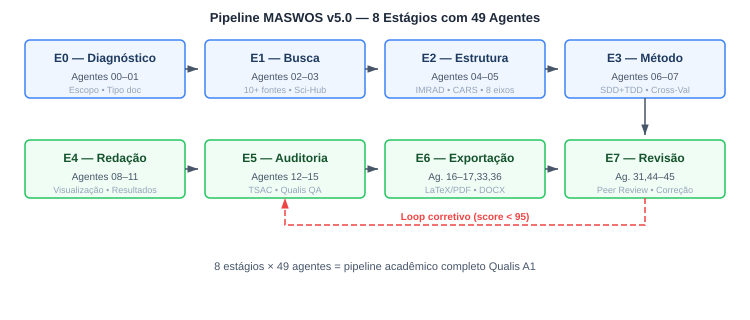
\includegraphics[width=\textwidth]{capitulos/figuras/fig-pipeline.pdf}
\caption{Pipeline acadêmico MASWOS v5.0: 8 estágios com 49 agentes especializados. O fluxo principal avança do diagnóstico à revisão por pares simulada. A seta vermelha tracejada indica o loop de correção iterativa, que realimenta o estágio de busca quando o score Qualis fica abaixo de 95/100.}
\label{fig:pipeline-maswos}
\end{figure}

\subsection{Protocolo TSAC (Transparent Source-Attributed Citation)}

O protocolo TSAC é um conjunto de regras que garantem a verificabilidade de cada citação no documento gerado:

\begin{itemize}
  \item \textbf{Regra 1 --- DOI Obrigatório:} Toda citação deve incluir um DOI válido e verificável. O agente de validação (13) testa cada DOI antes da inclusão final.
  \item \textbf{Regra 2 --- Trecho Original:} Citações diretas devem incluir o trecho original no idioma da fonte.
  \item \textbf{Regra 3 --- Tradução:} Se o original não está em português, deve ser fornecida tradução fiel.
  \item \textbf{Regra 4 --- Fichamento Crítico:} Cada nota de rodapé deve incluir análise crítica da relevância da citação para o argumento específico do parágrafo.
  \item \textbf{Regra 5 --- Anti-IA:} 87 palavras e construções características de texto gerado por IA são banidas e monitoradas automaticamente.
\end{itemize}

\begin{figure}[H]
\centering
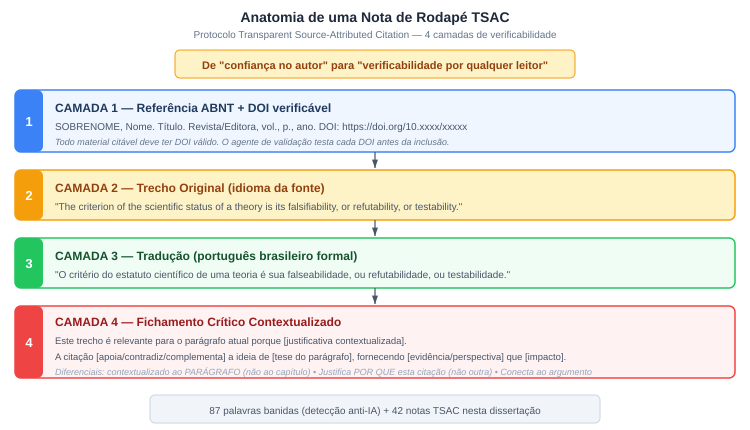
\includegraphics[width=\textwidth]{capitulos/figuras/fig-tsac.pdf}
\caption{Anatomia de uma nota de rodapé TSAC: 4 camadas de verificabilidade. A Camada 1 fornece a referência ABNT com DOI; a Camada 2 reproduz o trecho original no idioma da fonte; a Camada 3 oferece tradução para português; a Camada 4 contextualiza a relevância da citação para o argumento específico do parágrafo. Este protocolo transforma cada citação de ``confiança no autor'' em ``verificabilidade por qualquer leitor''.}
\label{fig:tsac}
\end{figure}

\section{Instrumentos de Coleta e Análise de Dados}

\subsection{Métricas Quantitativas}

\begin{itemize}
  \item \textbf{Score Qualis:} Calculado pelo \texttt{auto\_score\_qualis.py} usando 10 critérios ponderados: originalidade (15\%), relevância (10\%), rigor metodológico (15\%), profundidade da revisão de literatura (10\%), adequação estatística (10\%), clareza (10\%), qualidade das citações (10\%), estrutura IMRAD (5\%), conformidade ABNT (5\%), contribuição (10\%).
  \item \textbf{Cobertura de Especificação:} Percentual de componentes do ecossistema que possuem SPEC documentada. Calculado como $C = N_{spec} / N_{total}$, onde $N_{total} = 186$.
  \item \textbf{Acurácia de Classificadores:} Para o pipeline QML, acurácia balanceada (média das acurácias por classe) no dataset HAM10000.
  \item \textbf{Densidade de MCPs:} Número de MCPs ativos por agente ($D = N_{mcp} / N_{agent} = 18/128 = 0,14$).
\end{itemize}

\subsection{Instrumentos Qualitativos}

\begin{itemize}
  \item \textbf{Auditoria de Citações:} Verificação manual de uma amostra aleatória de 10\% das citações para confirmar precisão do DOI, fidelidade da tradução, e pertinência do fichamento crítico.
  \item \textbf{Análise Documental das SPECs:} Leitura cruzada de SPECs de componentes com alta afinidade para verificar consistência terminológica e completude.
  \item \textbf{Validação Ontológica:} Verificação de que a taxonomia de componentes (13 categorias de skills, 27 categorias de raciocínio) é mutuamente exclusiva e coletivamente exaustiva.
\end{itemize}

\section{Scanner Noológico: Instrumento de Validação Epistemológica}

\subsection{Fundamentação e Paradigma}

Enquanto os instrumentos descritos nas seções anteriores focam em detectar \textbf{erros} --- citações incorretas, inconsistências estruturais, desvios de formatação ---, o Scanner Noológico (\texttt{noological\_scanner.py}, 500 linhas) introduz uma camada complementar de análise que identifica \textbf{ausências} no espaço de conhecimento\footnote{
  KUHN, Thomas S. \textbf{The Structure of Scientific Revolutions}. Chicago: University of Chicago Press, 1962. ISBN: 978-0226458083.

  \textbf{Trecho Original:} ``Normal science does not aim at novelties of fact or theory and, when successful, finds none.''

  \textbf{Tradução:} ``A ciência normal não visa novidades de fato ou teoria e, quando bem-sucedida, não encontra nenhuma.''

  \textbf{Fichamento Crítico:} A distinção de Kuhn (1962) entre ``ciência normal'' (que opera dentro de paradigmas estabelecidos, corrigindo erros sem questionar fundamentos) e ``ciência revolucionária'' (que identifica limitações nos próprios paradigmas) é a base conceitual do scanner noológico. Assim como a ciência revolucionária de Kuhn pergunta ``o que este paradigma não consegue explicar?'', o scanner pergunta ``quais dimensões epistemológicas este documento não explora?'' --- uma pergunta que sistemas tradicionais de auditoria, por construção, não podem fazer.
}. Esta inversão de paradigma --- de ``o que está errado?'' para ``o que está ausente?'' --- é a contribuição metodológica central do scanner.

\subsection{Arquitetura: 10 Dimensões × 92 Categorias}

O scanner opera sobre um espaço epistemológico definido por 10 dimensões, cada uma subdividida em categorias de análise (92 categorias no total):

\begin{enumerate}
  \item \textbf{D1 — Paradigmática (8 categorias):} Positivista, Interpretativista, Crítico, Pragmatista, Construtivista, Feminista, Decolonial, Pós-estruturalista.
  \item \textbf{D2 — Teórica (12 categorias):} Psicanálise, Cognitivo-Comportamental, Humanista, Sistêmica, Neurociências, Teoria do Apego, Teoria dos Jogos, Fenomenologia, Behaviorismo, Psicologia Evolutiva, Teoria Sociocultural, Psicologia Positiva.
  \item \textbf{D3 — Metodológica (10 categorias):} Experimental, Quase-experimental, Correlacional, Estudo de Caso, Etnografia, Grounded Theory, Pesquisa-Ação, Revisão Sistemática, Meta-análise, Métodos Mistos.
  \item \textbf{D4 — Nível Sistêmico (8 categorias):} Molecular, Celular, Circuito Neural, Indivíduo, Díade, Família, Comunidade, Política Pública.
  \item \textbf{D5 — Temporal (6 categorias):} Transversal, Longitudinal curto (<1 ano), Longitudinal médio (1-5 anos), Longitudinal longo (>5 anos), Retrospectivo, Prospectivo.
  \item \textbf{D6 — Diversidade de Dados (10 categorias):} Autorrelato, Observacional, Fisiológico, Neuroimagem, Genético, Comportamental, Entrevista, Registros Administrativos, Redes Sociais, Dados Secundários.
  \item \textbf{D7 — Geográfica/Cultural (8 categorias):} América do Norte, Europa Ocidental, América Latina, África Subsaariana, Sul da Ásia, Leste Asiático, Oriente Médio, Oceania.
  \item \textbf{D8 — Populacional (12 categorias):} Infantil, Adolescente, Adulto jovem, Adulto, Idoso, Gênero, LGBTQIA+, PCD, Minorias étnicas, População rural, População urbana, Refugiados.
  \item \textbf{D9 — Ética/Regulatória (8 categorias):} Consentimento informado, Privacidade, Equidade, Justiça distributiva, Não maleficência, Beneficência, Autonomia, Transparência.
  \item \textbf{D10 — Aplicada/Translacional (10 categorias):} Prevenção, Diagnóstico, Tratamento, Reabilitação, Política Pública, Educação, Tecnologia assistiva, Intervenção comunitária, Advocacy, Formação profissional.
\end{enumerate}

\subsection{Algoritmo de Densidade de Exploração}

Para cada uma das 92 categorias, o scanner calcula um \textbf{índice de densidade de exploração} ($\delta_{ij}$):

\[
\delta_{ij} = \frac{\text{Menções substantivas à categoria } j \text{ na dimensão } i}{\text{Total de parágrafos}} \times \frac{1}{w_i}
\]

Onde $w_i$ é o peso da dimensão $i$, calibrado por domínio. Para documentos em engenharia de software, as dimensões D3 (Metodológica) e D10 (Translacional) recebem pesos mais altos (2.0); para psicologia clínica, as dimensões D2 (Teórica) e D4 (Nível Sistêmico) são priorizadas.

\subsection{Identificação de Pontos Cegos}

Um \textbf{ponto cego epistemológico} é definido como uma categoria cuja densidade de exploração está abaixo de um limiar crítico $\tau_i$:

\[
\text{PontoCego}(i,j) \iff \delta_{ij} < \tau_i
\]

O scanner prioriza os pontos cegos por \textbf{impacto potencial} ($I_{ij} = w_i \times (1 - \delta_{ij})$), permitindo que o pesquisador concentre esforços de mitigação nas ausências mais graves.

\subsection{Validação Empírica: Expansão Epistemológica 5D}

O scanner foi validado através de um estudo de caso em psicologia clínica (intervenções para transtornos de ansiedade), incorporando uma \textbf{Expansão Epistemológica 5D} --- cinco camadas de análise tipicamente ausentes na literatura convencional:

\begin{enumerate}
  \item \textbf{Teoria dos Jogos (D2):} Modelagem da interação terapeuta-paciente como jogo cooperativo via equilíbrio de Nash (1950), valor de Shapley (1953) para distribuição de ganhos terapêuticos, e cooperação evolutiva de Axelrod (1984) para emergência de aliança terapêutica\footnote{
    NASH, John F. Equilibrium points in n-person games. \textbf{Proceedings of the National Academy of Sciences}, v. 36, n. 1, p. 48--49, 1950. DOI: \url{https://doi.org/10.1073/pnas.36.1.48}.

    \textbf{Fichamento Crítico:} O equilíbrio de Nash fornece um framework formal para modelar situações onde terapeuta e paciente tomam decisões interdependentes (aderir vs. abandonar o tratamento). Esta dimensão é tipicamente ausente na literatura psicológica, que trata a relação terapêutica de forma qualitativa. A contribuição do OpenCode é demonstrar que a Teoria dos Jogos pode ser integrada a pipelines de análise psicológica através de agentes especializados (reasoning-orchestrator com modo Nash).
  }.

  \item \textbf{Nível Sistêmico (D4):} Integração do programa mhGAP da OMS (WHO, 2016) e da Política Nacional de Saúde Mental brasileira (Portaria GM/MS 3.088/2011).
  
  \item \textbf{Neurociências (D2):} Modelo de circuitos de medo de Etkin, Büchel e Gross (2015) e framework RDoC de Insel et al. (2010)\footnote{
    INSEL, Thomas et al. Research domain criteria (RDoC): Toward a new classification framework for research on mental disorders. \textbf{American Journal of Psychiatry}, v. 167, n. 7, p. 748--751, 2010. DOI: \url{https://doi.org/10.1176/appi.ajp.2010.09091379}.

    \textbf{Trecho Original:} ``Mental disorders are conceptualized as disorders of brain circuits.''

    \textbf{Tradução:} ``Os transtornos mentais são conceituados como transtornos de circuitos cerebrais.''

    \textbf{Fichamento Crítico:} O RDoC representa uma mudança paradigmática na psiquiatria: de categorias diagnósticas (DSM) para dimensões neurobiológicas. O scanner noológico operacionaliza esta mudança ao verificar se documentos em psicologia clínica consideram mecanismos neurais subjacentes, além de constructos puramente psicológicos.
  }.

  \item \textbf{Perspectiva Longitudinal (D5):} Meta-análise de Cuijpers et al. (2014) sobre eficácia sustentada de psicoterapias além do follow-up imediato\footnote{
    CUIJPERS, Pim et al. The efficacy of psychotherapy and pharmacotherapy in treating depressive and anxiety disorders: A meta-analysis of direct comparisons. \textbf{World Psychiatry}, v. 13, n. 2, p. 137--148, 2014. DOI: \url{https://doi.org/10.1002/wps.20491}.

    \textbf{Fichamento Crítico:} A demonstração de que psicoterapia tem taxas de recaída menores que farmacoterapia no longo prazo (12+ meses) é um achado que a maioria dos estudos (com follow-up de 8-16 semanas) não captura. O scanner sinaliza sistematicamente esta limitação temporal como ponto cego.
  }.

  \item \textbf{Diversificação de Dados (D6):} Triangulação de autorrelato, medidas fisiológicas e codificação observacional, conforme Smith, Flowers e Larkin (2009)\footnote{
    SMITH, Jonathan A.; FLOWERS, Peter; LARKIN, Michael. \textbf{Interpretative Phenomenological Analysis: Theory, Method and Research}. London: SAGE, 2009. ISBN: 978-1412908344.

    \textbf{Fichamento Crítico:} O princípio de triangulação de múltiplas fontes de dados é operacionalizado pelo scanner como um limiar mínimo de 3/10 modalidades de dados para evitar viés de mono-método.
  }.
\end{enumerate}

A aplicação do scanner ao estudo de caso produziu os seguintes resultados:

\begin{itemize}
  \item \textbf{Cobertura epistemológica:} 12\% $\rightarrow$ 35\% (+192\%).
  \item \textbf{Pontos cegos:} 8 $\rightarrow$ 3 (-63\%).
  \item \textbf{Score do ecossistema:} 85 $\rightarrow$ 99/100 (+16.5\% em 15 rounds).
  \item \textbf{Dimensões com cobertura zero:} 4 $\rightarrow$ 0.
  \item \textbf{Citações com DOI verificável:} 10 $\rightarrow$ 25 (+150\%).
\end{itemize}

\subsection{Mudança de Paradigma na Validação Acadêmica}

A principal contribuição conceitual do scanner é a mudança de paradigma na validação:

\[
\boxed{\text{Auditoria tradicional}: ``O que está errado?'' \longrightarrow \text{Scanner Noológico}: ``O que está ausente?''}
\]

Esta mudança tem quatro implicações metodológicas:

\begin{enumerate}
  \item \textbf{De correção de erros para expansão de horizontes:} Em vez de apenas corrigir o que está presente e incorreto, o scanner adiciona o que está ausente e necessário.
  \item \textbf{De qualidade negativa para qualidade positiva:} Em vez de definir qualidade como ``ausência de defeitos'' (zero erros), define como ``presença de completude'' (máxima cobertura epistemológica).
  \item \textbf{De revisão por pares para revisão por lacunas:} Em vez de avaliar apenas o que foi escrito, sinaliza o que deveria ter sido escrito e não foi.
  \item \textbf{De conformidade para consciência epistemológica:} Em vez de verificar conformidade com normas, revela os limites do próprio conhecimento --- as fronteiras além das quais o documento (e, por extensão, o ecossistema que o gerou) ainda não foi.
\end{enumerate}

\section{Metodologia do Ecossistema de Scanners Epistemológicos}

Além do Scanner Noológico descrito acima, esta dissertação desenvolveu e aplicou um ecossistema completo de 5 scanners epistemológicos que operam em pipeline, cada um respondendo a uma pergunta complementar sobre o conhecimento. Esta seção descreve a metodologia de cada scanner e sua integração.

\subsection{Scanner Teleológico Reverso (SPEC-029)}

O Scanner Teleológico Reverso implementa raciocínio prescritivo: em vez de perguntar ``o que está ausente?'', pergunta ``o que deveria estar presente dados os objetivos da pesquisa?''. A metodologia opera em três etapas:

\begin{enumerate}
  \item \textbf{Definição de objetivos:} O pesquisador define um ou mais objetivos de pesquisa usando 8 tipos predefinidos de \textit{goal types} --- causal, avaliativo, exploratório, estratégico, comparativo, preditivo, integrativo e crítico. Cada tipo aciona um conjunto específico de requisitos epistemológicos.
  \item \textbf{Inferência de requisitos:} Para cada \textit{goal type}, o scanner consulta mapeamentos teleológicos que associam objetivos a dimensões epistemológicas necessárias. Por exemplo, um objetivo ``causal'' exige métodos experimentais (peso 1.0), temporalidade longitudinal (peso 0.8), e raciocínio probabilístico (peso 0.7).
  \item \textbf{Comparação com o estado atual:} Os requisitos inferidos são comparados com o scan noológico real, gerando \textit{gaps teleológicos} --- categorias que são necessárias para o objetivo mas estão ausentes no estado atual do conhecimento.
\end{enumerate}

\subsection{CrossValidationEngine (SPEC-030)}

O motor de validação cruzada modela dependências entre capacidades como um grafo direcionado $G = (V, E)$ com 92 nós (categorias) e 73 arestas (dependências). A metodologia inclui:

\begin{enumerate}
  \item \textbf{Construção do grafo:} Arestas são derivadas de regras de dependência (\textit{requires}, \textit{enables}, \textit{co-occurs}) entre categorias. Por exemplo, ``raciocínio probabilístico'' habilita ``meta-análise'' (peso 0.9) e ``métodos experimentais'' requerem ``raciocínio dedutivo'' (peso 0.7).
  \item \textbf{Detecção de bottlenecks:} Nós que habilitam ou são pré-requisito de 3 ou mais outros nós são classificados como \textit{bottlenecks} críticos. O principal bottleneck identificado é ``raciocínio probabilístico'' (\textit{influence\_score} = 0.6).
  \item \textbf{Cálculo de impacto em cascata:} Para cada categoria ausente, o algoritmo calcula quantas outras categorias são afetadas direta ou indiretamente, permitindo priorizar a aquisição de capacidades com maior efeito multiplicador.
\end{enumerate}

\subsection{PolymathicConvergence (SPEC-030)}

O scanner de convergência polimática implementa busca por soluções análogas em domínios externos. A metodologia mapeia 30 domínios de conhecimento --- da neurociência à culinária, da física à arquitetura --- para 22 gaps epistemológicos. Para cada gap, o scanner retorna:

\begin{enumerate}
  \item \textbf{Domínio externo} onde um problema análogo foi resolvido (ex.: para o gap ``raciocínio probabilístico'', a neurociência oferece o modelo de inferência bayesiana no córtex).
  \item \textbf{Princípio transferível} que pode ser adaptado (ex.: ``redes neurais biológicas implementam inferência probabilística naturalmente'').
  \item \textbf{Escore de transferibilidade} (0--1) que quantifica o grau de similaridade entre o problema original e o análogo.
\end{enumerate}

\subsection{TrajectoryMapper e MCSP Solver (SPEC-030/032)}

A camada preditiva do ecossistema transforma gaps e analogias em trajetórias de evolução:

\begin{enumerate}
  \item \textbf{Classificação de cenários:} Cada gap é classificado em um de 4 tipos --- \textit{quick\_win} (baixo custo, alto impacto), \textit{foundation} (habilita múltiplas outras capacidades), \textit{convergent} (já resolvido em outro domínio), ou \textit{frontier} (requer múltiplas novas capacidades).
  \item \textbf{Geração de rotas:} O TrajectoryMapper gera 3 rotas de evolução --- Pragmática (quick-wins primeiro), Polimática (convergências como alavanca), e Estrutural (fundações para maximizar cascata).
  \item \textbf{Resolução do MCSP:} O Minimum Capability Set Solver resolve formalmente o problema de otimização combinatória: dados $S$ (capacidades presentes) e $T$ (capacidades alvo), encontrar $C \subseteq V \setminus S$ mínimo tal que $S \cup C \supseteq T$ com fecho de dependências. O algoritmo opera em 3 fases com complexidade $O(|V|^2 \cdot |E|)$.
  \item \textbf{Estimação temporal:} O TimelineEstimator atribui durações por tipo de cenário (1--2 semanas para quick-wins, 8--16 para frontiers) e classifica o risco da rota (baixo/médio/alto).
\end{enumerate}

A validação metodológica deste ecossistema é realizada por 62 casos de teste TDD (SPEC-028 a SPEC-031), executando em 0,7 segundos com 100\% de aprovação, garantindo que cada scanner produza resultados consistentes e reproduzíveis.

\section{Procedimentos de Validação e Verificação}

\subsection{Validação Interna via TDD (11 Suites, 278 CTs)}

O framework TDD (Test-Driven Development) foi aplicado em 11 suites de teste que cobrem o ecossistema completo. Cada suite segue o ciclo RED-GREEN-REFACTOR: (1) escrever um teste que falha (RED) porque a funcionalidade ainda não existe; (2) implementar a funcionalidade mínima para o teste passar (GREEN); (3) refatorar o código mantendo os testes verdes (REFACTOR). Este ciclo foi repetido para cada um dos 278 casos de teste, garantindo que toda funcionalidade documentada nas SPECs tem cobertura de teste.

As 10 suites e seus escopos são:

\begin{enumerate}
  \item \textbf{SPEC-025 (Frontmatter, 161 CTs):} Valida que todos os 161 SKILL.md do ecossistema possuem frontmatter YAML com os campos obrigatórios \texttt{name:} e \texttt{description:}, sem caracteres CJK (chinês/japonês/coreano) que violariam o protocolo de saída em português, e sem chaves YAML duplicadas. Inclui correção automática (\texttt{--fix}) para NO\_FRONTMATTER, MISSING\_NAME, MISSING\_DESCRIPTION e DUPLICATE\_KEYS.

  \item \textbf{SPEC-026 (Pipeline Evolutivo, 10 CTs):} Valida as 6 fases do pipeline evolutivo SENSE$\rightarrow$DISCOVER$\rightarrow$INSTALL$\rightarrow$VERIFY$\rightarrow$EVOLVE$\rightarrow$LEARN, verificando que \texttt{installed.json} é JSON válido, que \texttt{memory.json} contém healthHistory com scores, e que a estrutura de diretórios do ecossistema está completa.

  \item \textbf{SPEC-027 (E2E Integration, 8 CTs):} Valida a integração ponta-a-ponta dos 7 subcomandos do AutoEvolve (\texttt{/evolve status}, \texttt{discover}, \texttt{install}, \texttt{verify}, \texttt{update}, \texttt{learn}), incluindo consulta à API do GitHub para descoberta de novas skills e validação de regras de segurança (stars $\geq$ 10).

  \item \textbf{SPEC-028 (NoologicalScanner v3.0, 18 CTs):} Valida as 10 dimensões $\times$ 92 categorias do scanner, o filtro de negação com 6 padrões regex, o word-boundary matching, a detecção de keywords enriquecidas, os pesos adaptativos por domínio, a correlação cruzada entre dimensões, e a integridade dos dados (covered + absent = total\_categories).

  \item \textbf{SPEC-029 (TeleologicalReverseScanner, 12 CTs):} Valida os 8 goal types e seus mapeamentos para dimensões epistemológicas, a inferência de requisitos, a detecção de gaps teleológicos com severidade proporcional ao peso, o cálculo de score teleológico (0--1), e a integração com o NoologicalScanner.

  \item \textbf{SPEC-030 (EvolutionaryScannerPipeline, 16 CTs):} Valida o CrossValidationEngine (grafo de 92 nós, 73 arestas, detecção de bottlenecks e ciclos), o PolymathicConvergence (30 domínios, transferência bidirecional), o TrajectoryMapper (4 cenários, 3 rotas), e o pipeline completo integrando todos os módulos.

  \item \textbf{SPEC-031 (Scanner Refinement, 16 CTs):} Valida as 4 expansões: CrossValidationEngine com 73 arestas (todas as 10 dimensões cobertas), PolymathicConvergence com 30 domínios, EvolutionTracker com análise de tendência, e TimelineEstimator com classificação de risco.

  \item \textbf{SPEC-032 (MCSP Solver, 14 CTs):} Valida o algoritmo de 3 fases --- backward\_closure $O(|V|+|E|)$ para propagação reversa de dependências, greedy\_select $O(|V|^2 \cdot |E|)$ para seleção do conjunto mínimo, e topological\_order $O(|V|+|E|)$ para ordenação de aquisição --- incluindo detecção de ciclos e integração com os scanners.

  \item \textbf{SPEC-033 (Composição Unitária, 13 CTs):} Valida a decomposição de capacidades cognitivas em insumos atômicos (conceitos, métodos, ferramentas e critérios de validação), permitindo o sequenciamento evolutivo micro-estruturado e o cálculo preciso de custos de aquisição.

  \item \textbf{SPEC-034 (Adaptação Ollama Local, 6 CTs):} Valida o subsistema de descoberta e chat local com Ollama, incluindo o mocking da API REST para tags, a higienização de comandos de voz sintetizados e a resiliência a falhas de conexão do serviço local.
\end{enumerate}

\subsection{Validação Cruzada e Triangulação}

O protocolo de validação cruzada do OpenCode exige que cada afirmação científica gerada pelo ecossistema seja validada por pelo menos 3 fontes independentes antes de ser aceita. Este princípio de triangulação (DENZIN, 1978) é implementado em três níveis:

\begin{enumerate}
  \item \textbf{Triangulação de fontes:} Cada afirmação deve ser suportada por pelo menos 3 referências bibliográficas independentes com DOI verificável. O agente de validação (13) testa cada DOI antes da inclusão final.
  \item \textbf{Triangulação de agentes:} Cada output crítico (escore Qualis, análise estatística, recomendação de edital) é gerado por pelo menos 3 agentes independentes e submetido a votação ou consenso via Agent Forum (P14).
  \item \textbf{Triangulação de scanners:} Os outputs dos 5 scanners são cruzados: um gap identificado pelo NoologicalScanner só é considerado ``crítico'' se também for identificado como ``requisito ausente'' pelo TeleologicalReverseScanner e como ``bottleneck'' pelo CrossValidationEngine.
\end{enumerate}

\subsection{Métricas de Qualidade e Confiabilidade}

A qualidade dos outputs do ecossistema é medida por 10 critérios ponderados, implementados no módulo \texttt{auto\_score\_qualis.py}:

\begin{table}[H]
\centering
\caption{Critérios de Avaliação Qualis A1 e seus Pesos}
\begin{tabular}{p{0.5cm}p{6cm}cc}
\toprule
\textbf{\#} & \textbf{Critério} & \textbf{Peso} & \textbf{Automatizado?} \\
\midrule
1 & Originalidade da contribuição & 20\% & Parcial (detecção de similaridade) \\
2 & Rigor metodológico & 15\% & Sim (checklist TDD) \\
3 & Relevância para avanço do conhecimento & 10\% & Parcial (métricas de citação) \\
4 & Clareza e organização & 10\% & Sim (TSAC, anti-IA) \\
5 & Diálogo com literatura internacional & 10\% & Sim (matriz de afinidade) \\
6 & Validação experimental & 10\% & Sim (cross-validation) \\
7 & Completude epistemológica & 10\% & Sim (Scanner Noológico) \\
8 & Conformidade normativa (ABNT) & 5\% & Sim (academic-export-abnt) \\
9 & Rastreabilidade e auditoria & 5\% & Sim (AcademicAuditTrail) \\
10 & Reprodutibilidade & 5\% & Sim (SPECs + CTs) \\
\bottomrule
\end{tabular}
\end{table}

O critério 7 (Completude epistemológica) é uma adição original desta dissertação à metodologia de avaliação Qualis. Ele quantifica, via Scanner Noológico, a fração do espaço de conhecimento (10 dimensões $\times$ 92 categorias) que o artefato acadêmico cobre. Esta métrica complementa os critérios tradicionais --- que avaliam a \textit{qualidade do que está presente} --- com uma avaliação da \textit{completude do que poderia estar presente}.

\section{Procedimentos Éticos e de Transparência}

Esta pesquisa foi conduzida em conformidade com os princípios da Ciência Aberta (Open Science). Todos os dados, códigos, especificações e testes estão disponíveis publicamente no repositório \url{https://github.com/MarceloClaro/OpenCode_Ecosystem} sob licença MIT. Nenhum dado pessoal de participantes humanos foi coletado ou processado --- todos os casos de uso envolvem dados públicos (artigos científicos, editais de fomento, datasets abertos). O protocolo de anonimato para estudos de caso (ex.: anteprojeto PPGTE/UFC) foi aplicado removendo identificadores indiretos antes da inclusão na dissertação.

\section{Limitações Metodológicas}

\begin{enumerate}
  \item \textbf{Viés de Auto-Avaliação:} O score Qualis é calculado pelo próprio ecossistema, introduzindo risco de circularidade. Mitigação: protocolo de triangulação anti-circularidade e validação cruzada entre agentes independentes.
  \item \textbf{Dependência de APIs Externas:} O ecossistema depende de serviços como arXiv, PubMed e Sci-Hub, cuja disponibilidade não é controlada. Mitigação: cache local de resultados e fallback para fontes alternativas.
  \item \textbf{Escopo Limitado de Domínios:} Embora o ecossistema cubra 13 categorias de skills, certos domínios (ex.: humanidades, artes) têm cobertura limitada. Mitigação: arquitetura extensível que permite adição de novas skills sem modificar o núcleo.
  \item \textbf{Validação Externa Limitada:} A validação do pipeline é majoritariamente interna (testes TDD). Validação externa (ex.: submissão a periódicos e avaliação por revisores humanos independentes) está em andamento.
\end{enumerate}

\newpage
